\documentclass[]{article}

\usepackage[utf8]{inputenc}
\usepackage[paperheight=0.9in,paperwidth=2.6in,margin=0in]{geometry}
\usepackage{tikz}
\usetikzlibrary{shapes,arrows,automata,calc}
\usepackage{color}

\usepackage{booktabs}  % nicer table borders 

\begin{document}

%\clearpage
%\thispagestyle{empty}

\tiny{
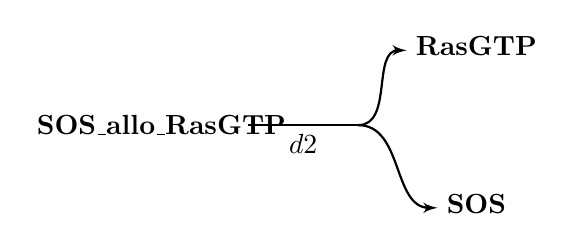
\begin{tikzpicture}[auto, outer sep=0pt, node distance=0cm,>=latex']

\node at (0, -1) (ALLO) {$\bf SOS\_allo\_RasGTP$};
\node at (4, 0) (RAS_GTP) {$\bf RasGTP$};
\node at (4, -2) (SOS) {$\bf SOS$};
\node at (2.5, -1) (MIDPOINT) {};
    \draw [-, thick] ($(MIDPOINT)$) to node {$d2$}
    ($(ALLO)+(1.1,0)$);
    \path [->, thick] ($(MIDPOINT)$) edge[in=180, out=0]
    ($(RAS_GTP.west)+(0,-0.05)$);
    \path [->, thick] ($(MIDPOINT)$) edge[in=180, out=0]
    ($(SOS.west)+(0, -0.05)$);
\end{tikzpicture} 
}

\end{document}

